\documentclass[letterpaper, 12 pt]{report}
\setcounter{secnumdepth}{0}	

\usepackage{color}
\usepackage{hyperref}
\usepackage[utf8]{inputenc}
\usepackage{graphicx}
\usepackage{subcaption}
\usepackage{float}

\hypersetup{
    colorlinks,
    linktoc=all,
    citecolor=black,
    filecolor=black,
    linkcolor=black,
    urlcolor=blue
}

% -------------------------------------------------------------------------------------
% BEGIN DOCUMENT
% -------------------------------------------------------------------------------------
\begin{document}
\title{VoiceClassifier User Manual}
\author{Andrew Omondi}
\date{August 2017}
\maketitle
\pagestyle{empty}

% -------------------------------------------------------------------------------------
% TABLE OF CONTENTS
% -------------------------------------------------------------------------------------
\tableofcontents
\newpage

% -------------------------------------------------------------------------------------
% PREFACE
% -------------------------------------------------------------------------------------
\section{Introduction}
\subsection{About this guide}
This document provides information about the functionality and use of the VoiceClassifier Android app.

\subsection{Audience}
This guide is intended for individuals who wish to take part in the collection of voice data  samples by use of the VoiceClassifier app and help in the improvement of its voice analysis methods.

\newpage


% -------------------------------------------------------------------------------------
% Overview of App
% -------------------------------------------------------------------------------------
\section{Overview of App}
VoiceClassfier is a simple android application that attempts to determine the gender of an individual from the collection of a 20 second voice sample from an individual. \\ \\
The user of the app can provide feedback for the result in the event an incorrect decision is made. This collected data will help in improving the app to help make future determinations better.  \\ \\
The app is intended to be simple to use and should provide little struggle for the user.

\newpage

\subsection{Launching the App}
To launch the app, tap the app icon on the home screen or menu screen of your  device.\\ \\
Launching of application will lead to a screen with a dialog with information detailing that a 20 second voice sample will be recorded on tapping the button as shown in Figure  \ref{fig:sub1}.\\ \\
Dismissing the dialog will result to a screen as shown in Figure \ref{fig:sub2}.\\ \\ \\ 

\begin{figure}[H]
\centering
\begin{subfigure}{.5\textwidth}
  \centering
  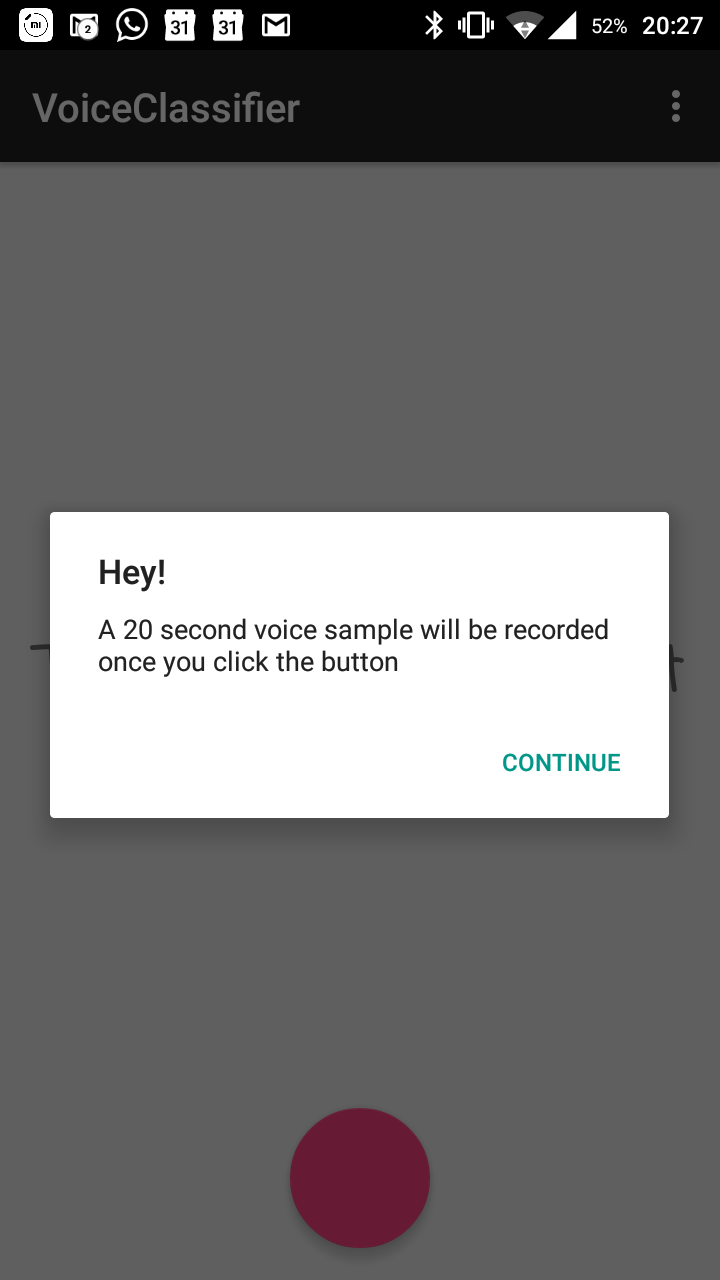
\includegraphics[width=.8\linewidth]{Photos/Opening_App.png}
  \caption{Info dialog on launch}
  \label{fig:sub1}
\end{subfigure}%
\begin{subfigure}{.5\textwidth}
  \centering
  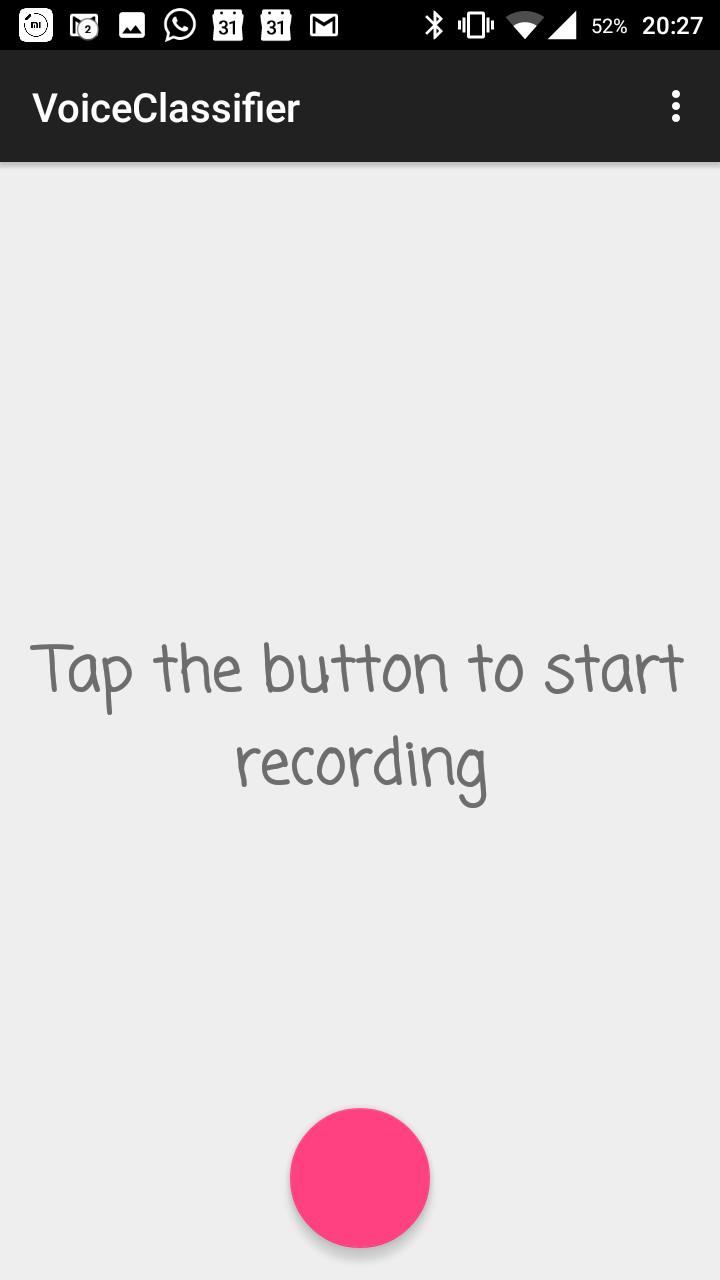
\includegraphics[width=.8\linewidth]{Photos/Opening_App_2.png}
  \caption{Default launch screen}
  \label{fig:sub2}
\end{subfigure}
\caption{Launching of the VoiceClassifier application}
\label{fig:launch}
\end{figure}

\newpage

\subsection{Recording Screen}
Once the user has tapped on the button, the application should begin recording the voice of the user.\\ \\ The recording sample is expected to be 20 seconds and the countdown will be shown on the screen as shown in Figure \ref{fig:countdown}.\\ \\ \\ 


\begin{figure}[H]
\centering
  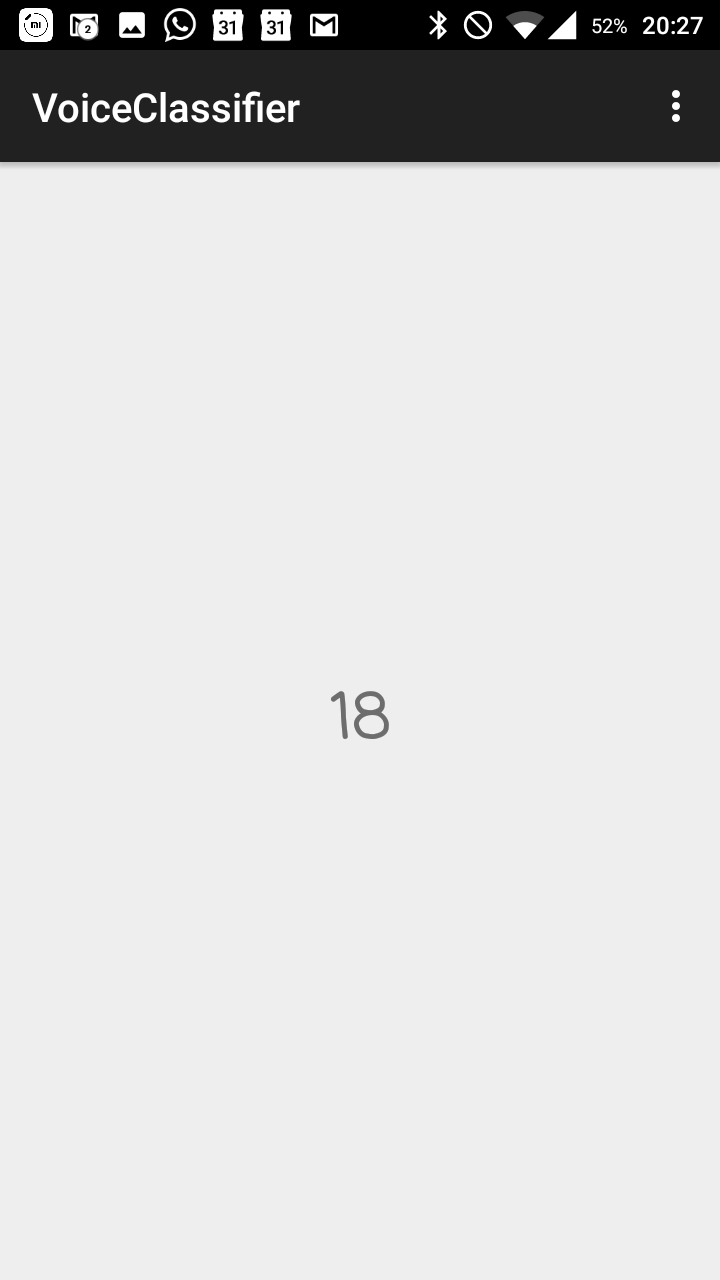
\includegraphics[width=0.45\linewidth]{Photos/Recording.png}
  \caption{Countdown screen while recording.}
\label{fig:countdown}
\end{figure}

\newpage

\subsection{Results}
Once the 20 second recording sample has been taken. The application will attempt to determine the gender of the voice sample recorded. \\ \\A graph of the pitch recorded over time will be shown on the result screen as shown in Figure \ref{fig:result}.\\ \\
\begin{figure}[H]
\centering
  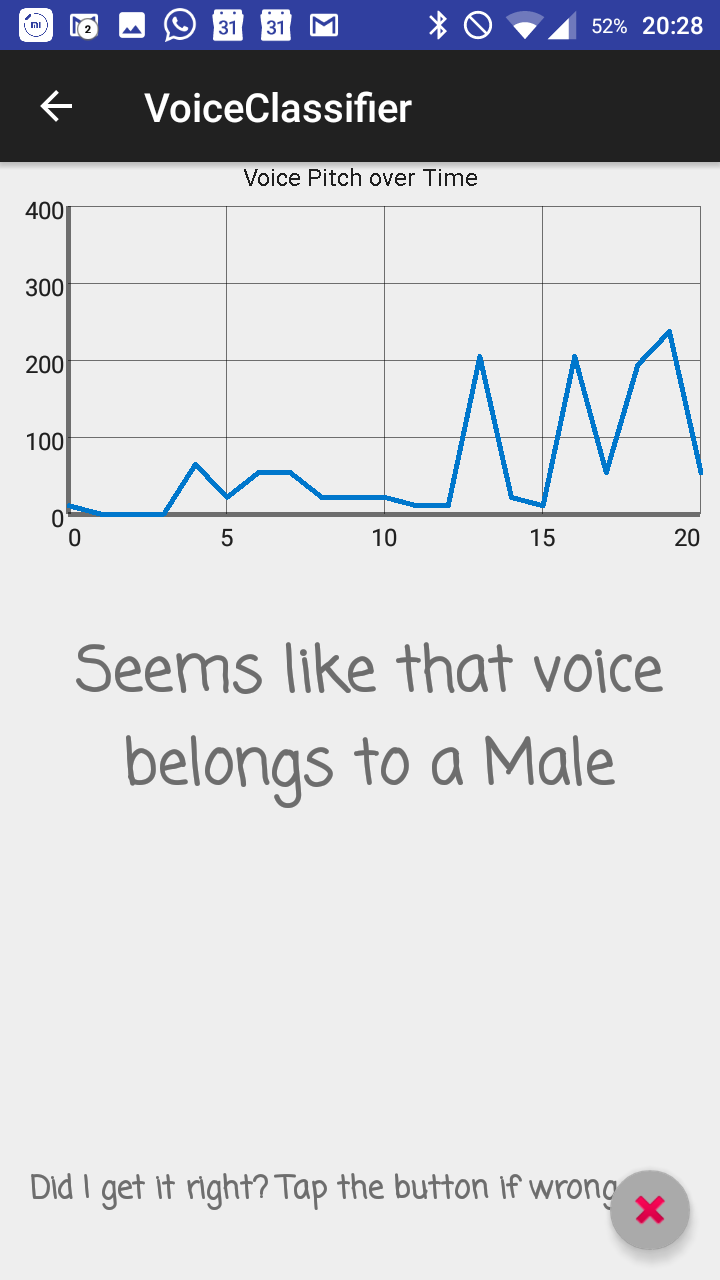
\includegraphics[width=0.45\linewidth]{Photos/Result.png}
  \caption{Analysis of recorded sample.}
\label{fig:result}
\end{figure}
The app will not always determine the right gender for the voice sample. In such a situation, the user can tap the button at the bottom of the result screen to give feedback to help improve the application.
\newpage

\section{Questions and Troubleshooting}
For any questions or issues with the VoiceClassfier Application, please contact the developer at : \href{mailto:andrueastman@gmail.com}{andrueastman@gmail.com} 

% -------------------------------------------------------------------------------------
% END DOCUMENT
% -------------------------------------------------------------------------------------
\end{document}